\subsection{External interfaces}
\subsubsection{User interfaces}
In this section, we report a mockup of the application’s User Interface. For the two types of users, Students and Educators, two different views are needed to guarantee all and only the desired functionalities for the two categories. Since coding on a smartphone’s keyboard is infeasible, computers are the main target of the application and the following User Interfaces are represented on a computer screen.\\
The Student UI allows the students to see the status of all the tournaments they are registered to, along with all the details regarding the battles within each tournament. Student must be able to join new battles by forming a team and see their ranking in the battle both before and after the closing deadline.\\
The Educator UI allows educators to create new tournaments and battles, invite other educators to post new battles in their tournaments and review the submissions of each time after the battle’s closing deadline, if required.\\
Note that this is only a representation of the user interface of the system and does not represent a final product.\\
\\
\textbf{Student UI}\\
\begin{figure}[htp!]
    \centering
    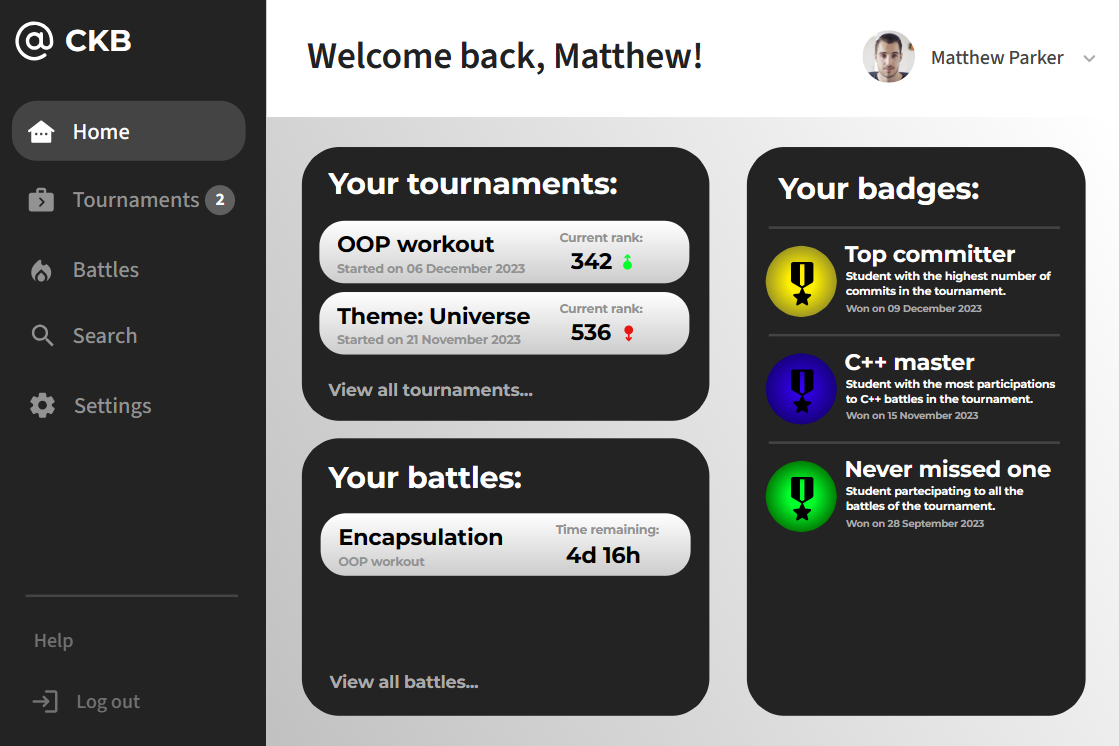
\includegraphics[width=0.9\linewidth]{Images/UI_Student_Home.png}
    \caption{Student Home screen}
    \label{fig:enter-label}
\end{figure}
\clearpage
\begin{figure}[h!]
    \centering
    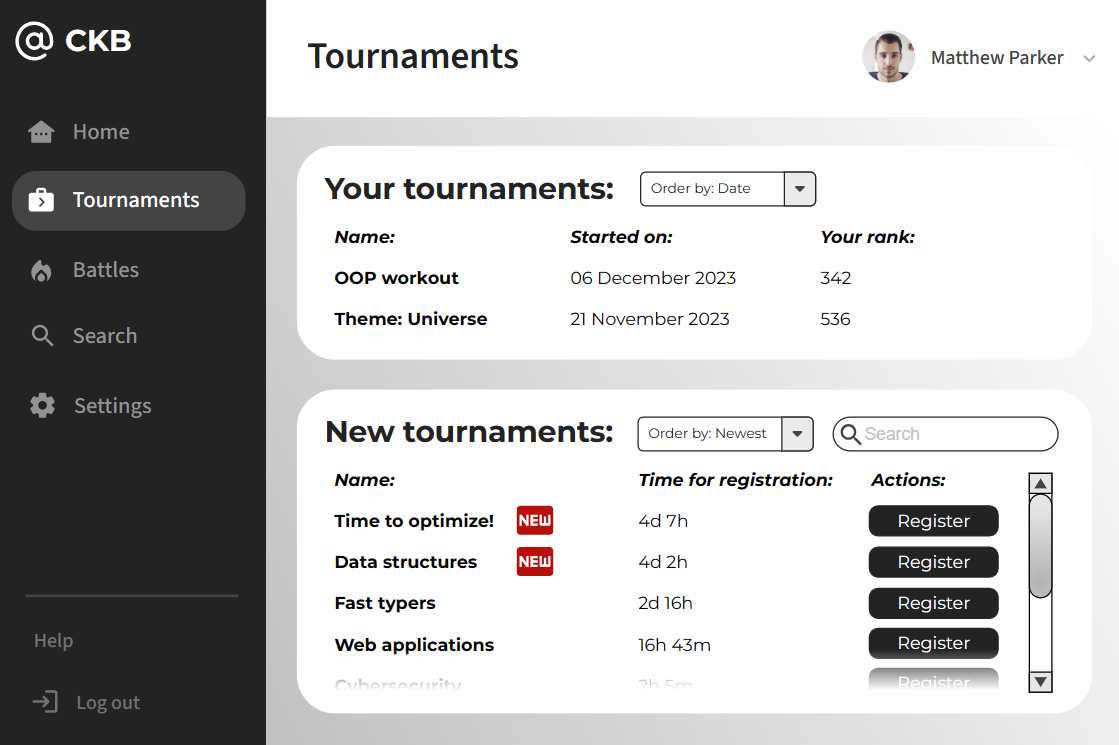
\includegraphics[width=0.9\linewidth]{Images/UI_Student_Tournaments.png}
    \caption{Student Tournaments screen}
    \label{fig:enter-label}
\end{figure}

\begin{figure}[h!]
    \centering
    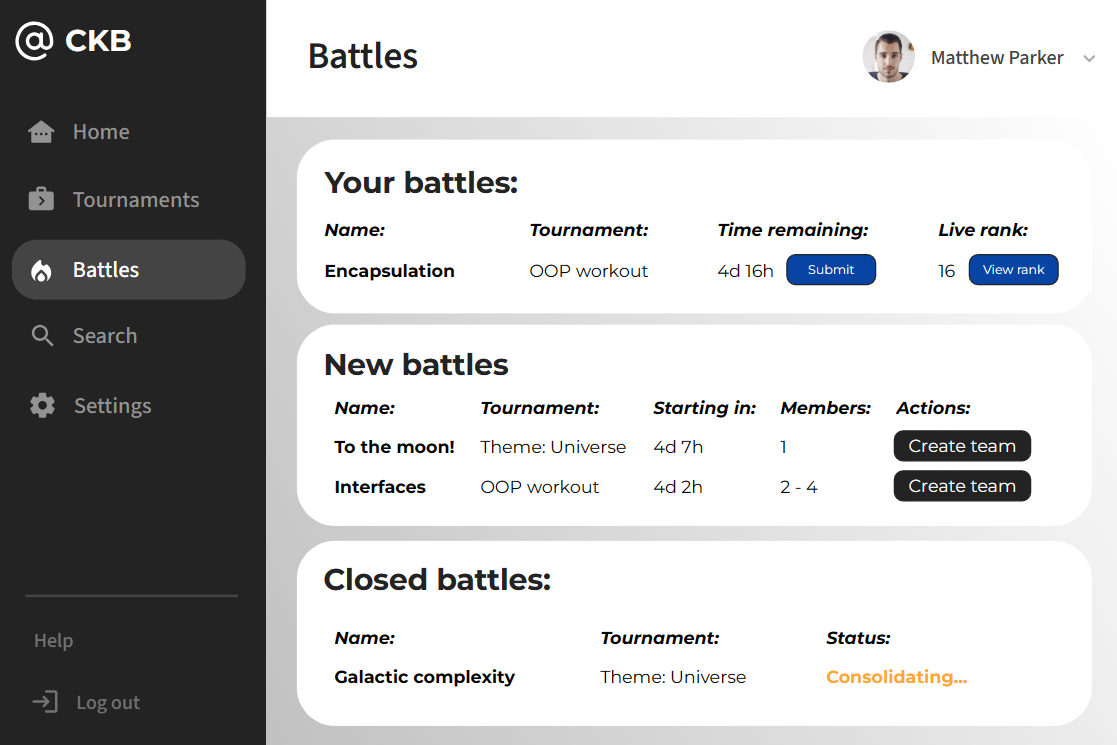
\includegraphics[width=0.9\linewidth]{Images/UI_Student_Battles.png}
    \caption{Student Battles screen}
    \label{fig:enter-label}
\end{figure}

\clearpage
\textbf{Educator UI}\\
\begin{figure}[h!]
    \centering
    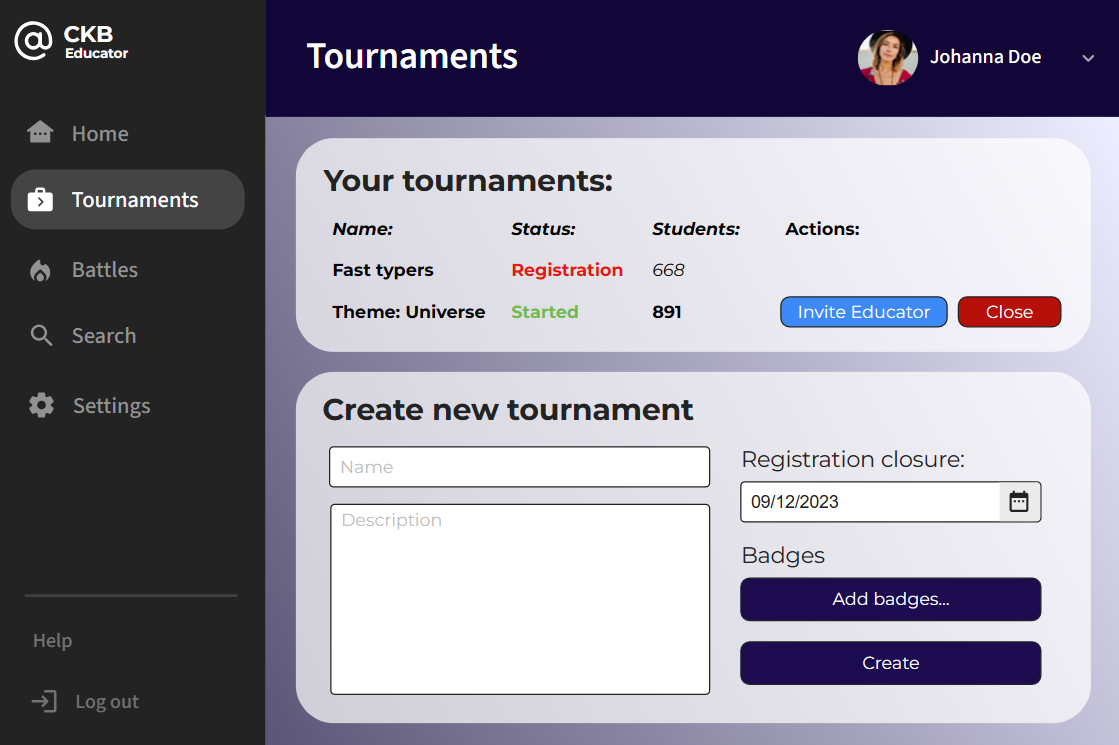
\includegraphics[width=0.85\linewidth]{Images/UI_Educator_Tournaments.png}
    \caption{Educator Tournaments screen}
    \label{fig:enter-label}
\end{figure}

\begin{figure}[h!]
    \centering
    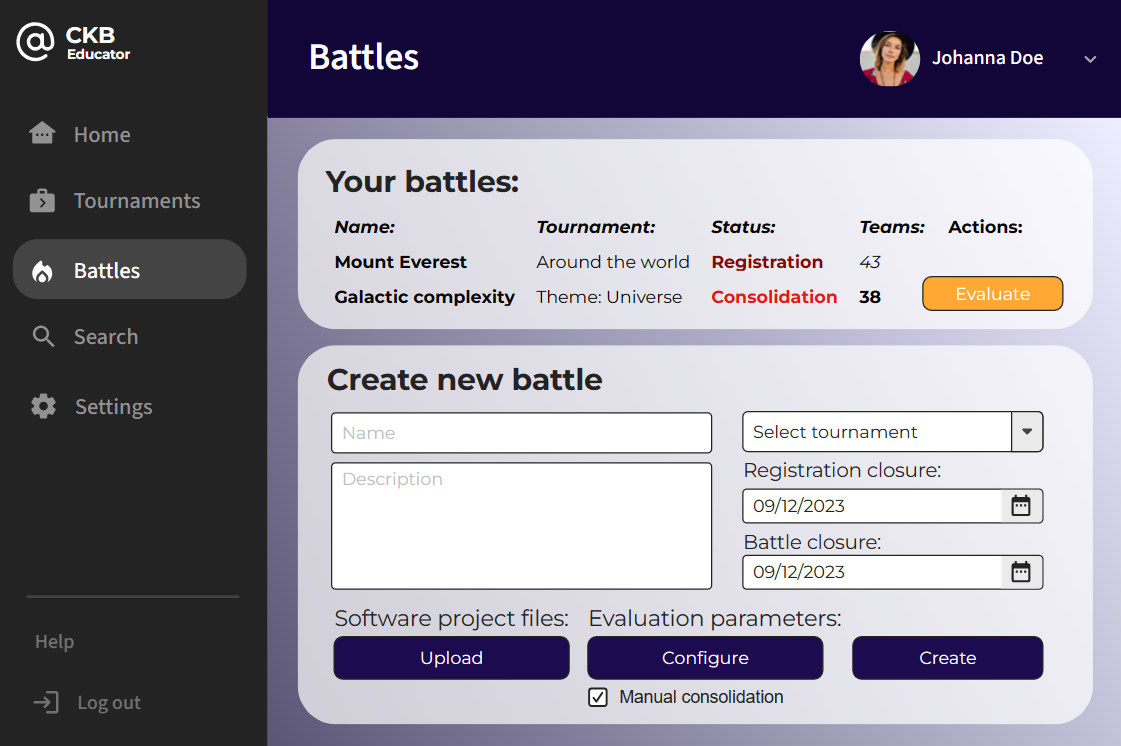
\includegraphics[width=0.85\linewidth]{Images/UI_Educator_Battles.png}
    \caption{Educator Battle screen}
    \label{fig:enter-label}
\end{figure}

\clearpage
\textbf{ }\\
\textbf{Badges Integration}\\
\\
Another important interface of the system is the one regarding the specification of the badges, along with the respective rules that must be met to earn the badge, happening during the creation of a tournament. The possible variables that can be exploited to decide whether to assign a badge or not are plenty, and it is not possible to define a-priori all of them. To solve this problem, the system offers a fixed set of variables, along with the possibility of defining new variables and new rules.\\
\\
The default variables are divided into two categories: student variables and global variables. The default rules consist of a comparison between the student's specific variable and the global variable. For example, assigning a badge to the student with the highest number of commits can be achieved in the following way:
\begin{figure}[H]
    \centering
    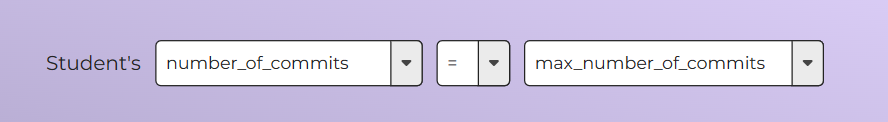
\includegraphics[width=0.9\linewidth]{Images/UI_Badge_form1.png}
    \caption{Student with maximum number of commits}
    \label{fig:UI_form1}
\end{figure}
As another example, assigning a badge to a student participating in all the battles in the tournament and reaching the first ten positions in the final tournament ranking can be performed in the following way:
\begin{figure}[H]
    \centering
    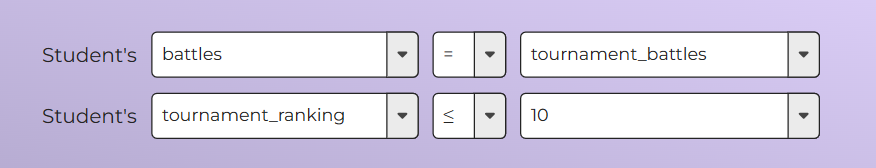
\includegraphics[width=0.9\linewidth]{Images/UI_Badge_form2.png}
    \caption{Student participating in all the battles and reaching the first ten positions in the tournament}
    \label{fig:UI_form2}
\end{figure}
The set of student variables, which will have a dedicated section explaining their meaning in the final application, is the following:

\begin{minted}{javascript}
    battles, //the number of battles in which the student participated
    battles_won, //the number of battles in which the student
                    //reached the first position in the final rank
    max_battle_ranking, //the maximum rank reached at the end of a battle
    max_commits, //maximum number of commits issued in a battle
    max_tournament_ranking, //the maximum rank reached during the tournament
    number_of_commits, //total number of commits issued by the student
    number_of_teammates, //total number of distinct teammates that
                        //participated with the student to the battles
    tournament_ranking, //the final rank of the student in the tournament
\end{minted}

The set of global variables, which will have a dedicated section explaining their meaning in the final application, is the following:

\begin{minted}{javascript}
    tournament_battles, //the number of battles in the tournament
    max_battles_won, //the maximum number of battles won
                    //by any student
    max_number_of_commits, //maximum number of commits issued by any student
    max_number_of_max_commits, //maximum number of commits issued
                                //by any student in a battle
\end{minted}

In addition to this set of variables, the system offers a way to define new variables by writing a JavaScript function that returns a number. The variables offered to the educator are the following:
\begin{minted}{javascript}
tournament
    .startTime //timestamp of the beginning of the tournament
    //timestamps are expressed as second elapsed since 00:00:00 of 1/1/1970 UTC
    .finishTime //timestamp of the beginning of the tournament
    .students[] //array of students
        .email //email of the student
        .finalRank //final rank of the student
        .ranks[] //rank of the student at the end of each battle
                //regardless if the student participated or not
    .battles[] //array of battles
        .startTime //timestamp of the beginning of the battle
        .finishTime //timestamp of the ending of the battle
        .languages[] //programming languages of the battle
        .registeredStudents[] //array of student emails
        .teams[] //array of teams
            .members[] //emails of members of the team
            .rank //final position in the rank of the battle
            .commits[] //array of commits:
                       //the last entry is the final submission
                .timestamp //timestamp of the submission
                .language //programming language used
                .author //student email
                .text[] //lines of code
\end{minted}

All the educator has to do is define a function that uses the previous data to return a quantity: if the function describes a student's variable, then the "student" object will be passed as a parameter.\\
\newpage
\textbf{ }\\
As an example, here is the process to describe the number of participations of each student in battles solvable with the programming language C\texttt{++}:

\begin{minted}{javascript}
function cpp_partecipations(student){
    let count = 0;
    for(let b of tournament.battles){
        if(b.registeredStudents.includes(student.email) && 
        b.languages.includes("C++")){
            count++;
        }
    }
    return count;
}
\end{minted}
After this, we can define a new global variable as the maximum number of participations in a C\texttt{++} battle by any student:

\begin{minted}{javascript}
function max_cpp_partecipations(){
    let max = 0;
    for(let s of tournament.students){
        let curr = cpp_partecipations(s);
        if(max < curr)
            max = curr;
    }
    return max;
}
\end{minted}
Once the two variables have been defined, the rule indicating the student with the most participations to C\texttt{++} battles can be expressed as above:

\begin{figure}[H]
    \centering
    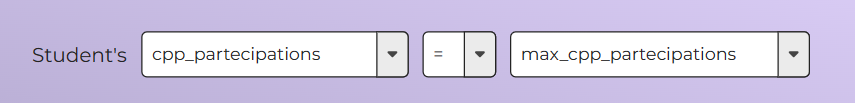
\includegraphics[width=0.9\linewidth]{Images/UI_Badge_form3.png}
    \caption{Student with the most participations to C\texttt{++} battles}
    \label{fig:UI_form3}
\end{figure}
We note that the scripts proposed by the educators will be executed in the same controlled environment as the student submissions, and badges with incorrect descriptions will be discarded.\\
\\
To add yet another layer of expressiveness, the system allows educators to define a rule function that directly returns if a student is eligible for a certain badge or not. To make a final example, here is the rule for selecting the students that issued two commits in less than a minute:
\newpage
\begin{minted}{javascript}
function two_commits_one_minute(student){
   for(let b of tournament.battles){
      for(let t of b.teams){
         if(t.members.includes(student.email)){
            for(let i=0; i<t.commits.length-1; i++){
               for(let j=i+1; j<t.commits.length &&
               t.commits[j].timestamp - t.commits[i].timestamp < 60; j++){
                  if(t.commits[i].author == student.email &&
                  t.commits[j].author == student.email){
                     return true;
                  }
               }
            }
         }
      }
   }
   return false;
}
\end{minted}
These are all the options that an educator has to describe the rules for assigning badges to students. The system offers both a simple, intuitive way to assign badges to students based on simple parameters and a more complex, expressive way of defining detailed rules. The scripts used for defining rules can be saved to be reused and shared among educators and many of them are offered as templates to make the draft of complex rules more intuitive, along with removing the strict need for educators to eventually learn JavaScript in depth just for this purpose.

\subsubsection{Hardware interfaces}
As the system functions as an online service accessible through standard web browsers, specific hardware interfaces are unnecessary. Users can interact with the system using any computer with good internet connectivity, eliminating the need for specialized hardware requirements.

\subsubsection{Software interfaces}
In order to provide all the desired services and functionalities, the system requires different software interfaces. The most important ones are the following:
\begin{itemize}
    \item
    GitHub Action: the system relies on GitHub Actions to automate the forwarding of the student commits to the system. GitHub Actions provides the required framework for continuous integration.
    \item
    Sandboxing: the system requires a robust sandboxing framework to execute external code in a secure and controlled environment. The primary purpose of this framework is to mitigate potential security risks associated with running untrusted code, ensuring the integrity and safety of the system. This framework is also needed to measure memory usage and execution time of the submitted scripts, in order to assess the quality of the submissions in case of an automated evaluation.
    \item
    Email Provider: the system requires an e-mail service provider to send confirmation e-mails to the users.
\end{itemize}

\subsection{Functional Requirements}

\begin{table}[H]
    \centering
    \begin{tabular}{|p{0.7cm}|p{15cm}|}
    \hline
        R1 & The system must allow users to register on the platform\\
    \hline
        R2 & The system must allow users to authenticate themselves and login securely\\
    \hline
        R3 & The system must allow educators to create new tournaments\\
    \hline
        R4 & Tournament creation must include specifying a description of the tournament\\
    \hline
        R5 & The system must allow authorized educators to create code kata battles within a tournament\\
    \hline
        R6 & Creation of CKB must include kata description, software project, build scripts, and scoring configurations\\
    \hline
        R7 & The system must allow students to register for individual battles or form teams based on specified team size limits\\
    \hline
        R8 & The system automatically creates GitHub repositories for battles \\
    \hline
        R9 & Students must be able to fork the repository and set up automated workflows using GitHub Actions\\
    \hline
        R10 & During the battle, the platform updates scores with every push made by students in real time\\
    \hline
        R11 & The system must allow educators to manually evaluate submissions\\
        \hline
        R12 & The system must allow authorized educators to add battles to tournaments\\
    \hline
        R13 & The battle closure triggers updates to personal tournament scores for each student\\
    \hline
        R14 & The system must allow educators to create badges associated with specific tournaments\\
    \hline
        R15 & Badges are automatically assigned based on predefined rules and student performance\\
    \hline
        R16 & The system automatically notifies students and educators about new tournaments, battles, and tournament closures\\
    \hline
        R17 & Notifications must include deadlines and updates\\
    \hline
        R18 & The system must allow the educator owning the tournament to authorize other educators to create CKB \\
    \hline
    \end{tabular}
    \caption{Functional requirements}
    \label{tab:requirements}
\end{table}


\subsubsection{Use cases diagrams}
In this section, an exploration of diverse use cases is presented to identify, elucidate, and organize the system's requirements. Each use case represents a series of interactions between users and the system, for them to achieve specific objectives. Actors involved in these scenarios, their actions, and reactions are here detailed, with potential exceptions leading to unsuccessful outcomes. To complement these descriptions, use case diagrams are employed, offering a visual representation of user-system interactions. These diagrams illustrate the user's actions, system functions executed by the application to fulfill user requests, and the given responses. Function names here provided are examples but maintain consistency across use cases to show the roles of the system’s components. In addition, logic units have been defined, these communicate with the Database Management System (DBMS) to execute the required actions.

\begin{enumerate}
   \item \textbf{Student Registration:}
After choosing the creation of a student account, a simple interface allows the student to register by inserting their email address, which needs to be unique within other students’ accounts. The format will be verified by the system and then an email containing a confirmation link that needs to be opened by the student to complete the registration is sent. They will be asked to also insert a unique username and a safe-enough password. After the registration process, a confirmation email is sent. The logical unit “UserManager” is a component of the system that communicates with DBMS to manage users’ registrations and logins.
   
   \begin{table}[H]
       \centering
       \begin{tabular}{|l|m{11cm}|}
        \hline
            Name & Registration of a student\\
        \hline
            Actors & Student, Email provider\\
        \hline
            Entry Condition & Student has access to the Internet and has not registered as a student in the system yet\\
        \hline
            Event Flow & 
            \begin{itemize}
                \item Student opens the web application
                \item Student clicks on the button "Sign Up as Student"
                \item System shows the registration form
                \item Student inserts username, email, and chosen password
                \item System checks inserted data
                \item System saves data and sends a confirmation email
                \item Student clicks on the received link
                \item System sends an email that confirms the subscription
            \end{itemize} \\
        \hline
            Exit Conditions & Registration has been successful: student's data are correctly inserted and saved into the system's database\\
        \hline
            Exceptions & Registration has not been successful if:
            \begin{itemize}
                \item Student inserts an already existing username or email
                \item Student inserts an unsafe password
            \end{itemize} \\
        \hline
       \end{tabular}
       \caption{UC1: Student Registration}
       \label{tab:uc1}
   \end{table}

   \newpage
   
   \item \textbf{Educator Registration:}
    After choosing the creation of an educator account, a simple interface allows the educator to register by inserting their email address, which needs to be unique within other educators’ accounts. The format will be verified by the system and then an email containing a confirmation link that needs to be opened by the educator to complete the registration is sent. They will be asked to also insert a unique username and a safe-enough password. After the registration process, a confirmation email is sent.
    
   \begin{table}[H]
       \centering
       \begin{tabular}{|l|m{11cm}|}
        \hline
            Name & Registration of an educator\\
        \hline
            Actors & Educator, Email provider\\
        \hline
            Entry Condition & Educator has access to the Internet and has not registered as an educator in the system yet\\
        \hline
            Event Flow & 
            \begin{itemize}
                \item Educator opens the web application
                \item Educator clicks on the button "Sign Up as Educator"
                \item System shows the registration form
                \item Educator inserts username, email, and chosen password
                \item System checks inserted data
                \item System saves data and sends a confirmation email
                \item Educator clicks on the received link
                \item System sends an email that confirms the subscription
            \end{itemize} \\
        \hline
            Exit Conditions & Registration has been successful: educator's data are correctly inserted and saved into the system's database\\
        \hline
            Exceptions & Registration has not been successful if:
            \begin{itemize}
                \item Educator inserts an already existing username or email
                \item Educator inserts an unsafe password
            \end{itemize} \\
        \hline
       \end{tabular}
       \caption{UC2: Educator Registration}
       \label{tab:uc2}
   \end{table}

   \newpage
   
   \item \textbf{Student Login:}
    Here we consider students' log in: they need to insert their credentials (email and password) and then, if they are valid, they are logged into the platform. Credentials’ validity is checked by the logical unit “UserManager”.

   \begin{table}[H]
       \centering
       \begin{tabular}{|l|m{11cm}|}
        \hline
            Name & Login of a student\\
        \hline
            Actors & Student\\
        \hline
            Entry Condition & Student has access to the Internet and has already registered as a student in the system\\
        \hline
            Event Flow & 
            \begin{itemize}
                \item Student opens the web application
                \item Student clicks on the button "Sign In as Student"
                \item System shows the login form
                \item Student inserts username and password
                \item System checks credentials
                \item System redirects to correct Home screen        
            \end{itemize} \\
        \hline
            Exit Conditions & Student logs in correctly: inserts correct credentials and sees correct web page\\
        \hline
            Exceptions & Student doesn't log in correctly if:
            \begin{itemize}
                \item Student inserts a nonexisting username
                \item Student inserts the wrong password
            \end{itemize} \\
        \hline
       \end{tabular}
       \caption{UC3: Student Login}
       \label{tab:uc3}
   \end{table}
   
   \newpage
   
   \item \textbf{Educator Login:}
    Here we consider the login to an educator account. The educator who wants to log in must be registered in the system. They need to insert their credentials (email and password) and then, if they are valid, they are logged into the platform.
    
   \begin{table}[H]
       \centering
       \begin{tabular}{|l|m{11cm}|}
        \hline
            Name & Login of an educator\\
        \hline
            Actors & Educator\\
        \hline
            Entry Condition & Educator has access to the Internet and has already registered as an educator in the system\\
        \hline
            Event Flow & 
            \begin{itemize}
                \item Educator opens the web application
                \item Educator clicks on the button "Sign In as Educator"
                \item System shows the login form
                \item Educator inserts username and password
                \item System checks credentials
                \item System redirects to correct Home screen        
            \end{itemize} \\
        \hline
            Exit Conditions & Educator logs in correctly: inserts correct credentials and sees correct web page\\
        \hline
            Exceptions & Educator doesn't log in correctly if:
            \begin{itemize}
                \item Educator inserts a nonexisting username
                \item Educator inserts a wrong password
            \end{itemize} \\
        \hline
       \end{tabular}
       \caption{UC4: Educator Login}
       \label{tab:uc4}
   \end{table}

   \newpage
   
   \item \textbf{Tournament Creation:}
    This use case considers the educator’s creation of a new tournament on the platform. Of course, to do this the educator needs to be logged into the platform. The educator inserts the name, description, and registration deadline. The “TournamentManager” logic unit is responsible for inserting the new tournament and its information into the database and communicating with the DBMS. All subscribed students are then notified about the newly inserted tournament.
    
   \begin{table}[H]
       \centering
       \begin{tabular}{|l|m{11cm}|}
        \hline
            Name & Creation of a tournament\\
        \hline
            Actors & Educator, Students\\
        \hline
            Entry Condition & Educator has already logged in\\
        \hline
            Event Flow & 
            \begin{itemize}
                \item Educator opens Tournament screen
                \item Educator writes name and description of the tournament
                \item Educator selects registration deadline
                \item Educator can add badges
                \item Educator clicks on the "Create" button
                \item System inserts new tournament's data into DB
                \item System shows the new tournament in the students' Tournaments screen
                \item System notifies subscribed students
            \end{itemize}\\
        \hline
            Exit Conditions & Tournament has been correctly created and inserted into DB, it's also visible to all students subscribed to the platform\\
        \hline
            Exceptions & Tournament has not been created if: 
            \begin{itemize}
                \item Tournament with an inserted name already exists
                \item Registration deadline is not valid
            \end{itemize}\\
        \hline
       \end{tabular}
       \caption{UC5: Tournament Creation}
       \label{tab:uc5}
   \end{table}
   
   \newpage
   
   \item \textbf{Add Battle Permission Granting:}
    After creating a tournament, the educator can grant other educators the possibility to add their battle to that tournament. The educator needs to be still logged into the platform and the other educators must exist. To do this, the educator uses a specific form where they can search for the educator they want to give permission to, inserting their email or their username. The “TournamentManager” will then insert this information into the database, communicating with the DBMS.
    
   \begin{table}[H]
       \centering
       \begin{tabular}{|l|m{11cm}|}
        \hline
            Name & Granting the permission to add a battle to a tournament\\
        \hline
            Actors & Educators\\
        \hline
            Entry Condition & Educator has already logged in and has created at least one tournament\\
        \hline
            Event Flow & 
            \begin{itemize}
                \item Educator opens Tournament screen
                \item Educator clicks on the "Invite Educator" button for the correct tournament
                \item System shows a specific form
                \item Educator searches for the other educator(s) they want to invite inserting their email or username
                \item System inserts tournament's new data into DB
            \end{itemize}\\
        \hline
            Exit Conditions & Other educator(s) have now the possibility to add their battle to the tournament\\
        \hline
            Exceptions & Permission is not given if: 
            \begin{itemize}
                \item Tournament is already closed or doesn't exist
                \item Educator is not the tournament's creator
                \item Inserted names or emails don't exist
                \item Selected educator has been already invited
            \end{itemize}\\
        \hline
       \end{tabular}
       \caption{UC6: Permission Granting}
       \label{tab:uc6}
   \end{table}
   
   \item \textbf{Battle Creation:}
    An educator can create a battle and add it to a tournament on the platform. To do this the educator must be logged in and have permission to insert a battle in that tournament.  
    The “TournamentManager” is responsible for checking if the educator can add their battle in that tournament on the DBMS. If they have permission, they can then use a form to upload the code kata, with a description and the software project, including test cases and build automation scripts, to set the minimum and maximum number of admitted students per group, the registration deadline, the final submission deadline and any additional configurations for scoring. All data are checked by the system and then inserted into the DB by a logic unit named “BattleManager”, that communicates with the DBMS.
    
   \begin{table}[H]
       \centering
       \begin{tabular}{|l|m{11cm}|}
        \hline
            Name & Creation of a battle\\
        \hline
            Actors & Educator, Subscribed students\\
        \hline
            Entry Condition & Educator has already logged in and has the permission to create a battle in that tournament\\
        \hline
            Event Flow & 
            \begin{itemize}
                \item Educator opens Battle screen
                \item Educator writes name and description of the battle
                \item Educator selects a tournament between the available ones
                \item Educator selects registration deadline and submission deadline 
                \item Educator clicks on the "Upload" button to upload the code kata, which includes test cases and build automation scripts
                \item Educator clicks on the "Configure" button to set group parameters and any additional configurations for evaluating
                \item Educator clicks on the "Create" button                
                \item System creates GitHub repository            
                \item System inserts battle's new data into DB
                \item System shows the new battle to Battles screen of students that are subscribed to that tournament 
                \item System sends a notification to subscribed students
            \end{itemize}\\
        \hline
            Exit Conditions & The battle is successfully created if students can see it and join it\\
        \hline
            Exceptions & Battle is not created if: 
            \begin{itemize}
                \item In that tournament already exists a battle with the same name
                \item The selected tournament is already closed
                \item Educator has not the permission to add a battle in that tournament
                \item Deadlines are inconsistent
                \item Code kata doesn't compile or tests are missing
            \end{itemize}\\
        \hline
       \end{tabular}
       \caption{UC7: Battle Creation}
       \label{tab:uc7}
   \end{table}

   \newpage

   \item \textbf{Tournament subscription:}
   A student can subscribe to a tournament. They must be logged into the platform and the tournament must be open. The “TournamentManager” inserts this information into the DBMS, so that after the subscription the student can be notified of all upcoming battles created within that tournament. 
   
   \begin{table}[H]
       \centering
       \begin{tabular}{|l|m{11cm}|}
        \hline
            Name & Subscribing to a tournament\\
        \hline
            Actors & Student\\
        \hline
            Entry Condition & Student has already logged in\\
        \hline
            Event Flow & 
            \begin{itemize}
                \item Student opens Tournament screen
                \item Student clicks on the "Register" button for the correct tournament
                \item System inserts subscription information into DB
                \item System puts the student into the notification list for that tournament's battle
                \item System shows the tournament in the student's Tournament screen
            \end{itemize}\\
        \hline
            Exit Conditions & Subscription went well when the student can now see the tournament they're subscribed to in his Home screen and can participate in its battles\\
        \hline
            Exceptions & Subscription fails if: 
            \begin{itemize}
                \item Tournament registration's deadline has expired
                \item Student is already subscribed to that tournament
            \end{itemize}\\
        \hline
       \end{tabular}
       \caption{UC8: Tournament subscription}
       \label{tab:uc8}
   \end{table}

   \newpage
   
   \item \textbf{Battle Join:}
   A student can join a battle if and only if they are subscribed to the tournament it belongs to and logged in. The “Tournament Manager” is responsible for checking if the student is subscribed to the tournament. When joining a battle, the student can choose between form a team with other students by sending them an invitation or doing it on their own. If the number of students in the formed team respects the set values then it’s accepted can participate in the competition. The “BattleManager” is the component that does this check. When the registration deadline expires, the platform creates a GitHub repository containing the code kata and sets GitHub Action's YAML file, then gives all students who joined permission to fork it and sends them the link.Students can start working on the project.
   
   \begin{table}[H]
       \centering
       \begin{tabular}{|l|m{11cm}|}
        \hline
            Name & Join a battle\\
        \hline
            Actors & Students\\
        \hline
            Entry Condition & Student has already logged in and is subscribed to the battle's tournament\\
        \hline
            Event Flow & 
            \begin{itemize}
                \item Student opens the Battle screen
                \item Student clicks on the "Create team" button for the correct battle
                \item Student can choose between inviting other subscribed students using the form shown by the system or joining it on their own
                \item System sends any team invitation and elaborates responses (see UC10)
                \item System checks if battle's team constraints are respected
                \item System inserts team's information into DB
                \item Team's students automatically join the battle
                \item System creates a GitHub repository containing the code kata and sets GHA's YAML file
                \item System gives permissions to fork the corresponding repository and sends the link to teams
                \item System shows the battle in the student's Battle screen                
            \end{itemize}\\
        \hline
            Exit Conditions & Students can see the battle in their Battle screen and can start working on the project\\
        \hline
            Exceptions & Students can't join the battle if: 
            \begin{itemize}
                \item Team is not accepted
                \item Battle registration's deadline has expired
            \end{itemize}\\
        \hline
       \end{tabular}
       \caption{UC9: Battle Join}
       \label{tab:uc9}
   \end{table}


   \newpage

   \item \textbf{Invitation accepting:}
   A student can receive the invitation to a team if and only if they are subscribed to the tournament it belongs to (this is checked when the invitation is sent by "TournamentManager"). The student can also choose to not accept the invitation.
   
   \begin{table}[H]
       \centering
       \begin{tabular}{|l|m{11cm}|}
        \hline
            Name & Accepting an invitation to a team\\
        \hline
            Actors & Student\\
        \hline
            Entry Condition & Student has received an invitation to a team\\
        \hline
            Event Flow & 
            \begin{itemize}
                \item Student logs in
                \item System shows to the student the invitation
                \item Student clicks on the "Accept" button
            \end{itemize}\\
        \hline
            Exit Conditions & The invitation is accepted, the student joins the team that needs to be checked (see UC9)\\
        \hline
            Exceptions & The student does not join the team if: 
            \begin{itemize}
                \item Student is not subscribed to the tournament
                \item Battle registration's deadline has expired
                \item Student doesn't accept the invitation
            \end{itemize}\\
        \hline
       \end{tabular}
       \caption{UC10: Invitation accepting}
       \label{tab:uc10}
   \end{table}

   \newpage
   
   \item \textbf{Code Manual Evaluation:}
    An educator can choose to manually evaluate the code of teams participating in a battle. To do so they must be logged in and they must be the creator of the battle. This is checked by the “BattleManager” component. The manual evaluation can be done only after the submission deadline has expired, in the consolidation stage. The educator uses the platform to go through each team’s sources.
    
   \begin{table}[H]
       \centering
       \begin{tabular}{|l|m{11cm}|}
        \hline
            Name & Evaluate manually the code of teams\\
        \hline
            Actors & Educator\\
        \hline
            Entry Condition & Educator has already logged in and has created at least one battle that is in the consolidation stage but not closed yet\\
        \hline
            Event Flow & 
            \begin{itemize}
                \item Educator opens the Battle screen
                \item Educator clicks the button "Evaluate" for the correct battle
                \item System shows each team's sources so that educators can go through them and evaluate them
                \item Educator inserts all grades
                \item System closes the battle
            \end{itemize}\\
        \hline
            Exit Conditions & The manual evaluation went well if the battle is closed and every team has a grade given by the educator that created the battle\\
        \hline
            Exceptions & The manual evaluation has failed if:
            \begin{itemize}
                \item Educator is not the creator of the battle
                \item Tournament is already closed
                \item Battle is already closed
            \end{itemize}\\
        \hline
       \end{tabular}
       \caption{UC11: Code Manual Evaluation}
       \label{tab:uc11}
   \end{table}

   \newpage
   
   \item \textbf{Tournament Closure:}
    An educator can close a tournament, but they must be not just logged into the platform, but they must be also the creator of that tournament and all the contained battles must be finished. The “TournamentManager” and the “BattleManager” are responsible for checking that. After the tournament is closed, the final tournament rank becomes available and the system notifies every participating student.
    
   \begin{table}[H]
       \centering
       \begin{tabular}{|l|m{11cm}|}
        \hline
            Name & Close a tournament\\
        \hline
            Actors & Educator, Subscribed students\\
        \hline
            Entry Condition & Educator has already logged in and has created at least one tournament that is not closed yet\\
        \hline
            Event Flow & 
            \begin{itemize}
                \item Educator opens Tournaments screen
                \item Educator clicks the button "Close" for the correct tournament
                \item System calculates final rank, registers it, and publishes it
                \item System notifies all subscribed students
            \end{itemize}\\
        \hline
            Exit Conditions & The tournament has been successfully closed, the final rank has been registered and published, and the subscribed users are correctly notified\\
        \hline
            Exceptions & The tournament is not successfully closed if:
            \begin{itemize}
                \item Educator is not the creator of the tournament
                \item Tournament is already closed
                \item One or more battles in the tournament have not been finished or completely evaluated yet
            \end{itemize}\\
        \hline
       \end{tabular}
       \caption{UC12: Tournament Closure}
       \label{tab:uc12}
   \end{table}

   \newpage
   
   \item \textbf{Badges Integration:}
    An educator, while creating a tournament, can also define gamification badges associated with it. They use a form on the platform that permits the inserting of the title and one or more rules that need to be fulfilled to obtain the badge. Rules can be chosen between predefined ones or created from scratch in JavaScript language. Since they are part of the tournament’s properties, the badges are inserted into the DB by the “TournamentManager” component.
    
   \begin{table}[H]
       \centering
       \begin{tabular}{|l|m{11cm}|}
        \hline
            Name & Create and add a badge\\
        \hline
            Actors & Educator\\
        \hline
            Entry Condition & Educator has already logged in and is creating a tournament\\
        \hline
            Event Flow & 
            \begin{itemize}
                \item Educator clicks the button "Add badge"
                \item System opens the form to create a badge
                \item Educator writes the title in the text box
                \item Educator writes rule(s) selecting correct variables to complete the equation they want or, if not present, writes a JavaScript code from scratch
                \item System saves the badge in DB
            \end{itemize}\\
        \hline
            Exit Conditions & The new badge is correctly saved in the DB and is syntactically correct\\
        \hline
            Exceptions & The badge is not accepted if:
            \begin{itemize}
                \item Exists another badge with the same title for that tournament
                \item Exists another badge with the same rule-set for that tournament
                \item JavaScript code is not syntactically correct
                \item Rules are mutually exclusive
                \item One or more rules are not achievable
            \end{itemize}\\
        \hline
       \end{tabular}
       \caption{UC13: Badges Integration}
       \label{tab:uc13}
   \end{table}
   
   \newpage

   \item \textbf{Badges Obtaining:}
    A student who is subscribed to a tournament can obtain the gamification badges of that tournament. They can win the badge by fulfilling all the corresponding rules. Each badge is assigned to one or more students at the end of the tournament. The set of badges corresponding to a tournament can be retrieved via the "TournamentManager" component. After obtaining a badge, it can be seen on the student’s profile, to do so the collected badges are inserted into the DB by the “UserManager” component.
    
   \begin{table}[H]
       \centering
       \begin{tabular}{|l|m{11cm}|}
        \hline
            Name & Student obtains a badge\\
        \hline
            Actors & Student \\
        \hline
            Entry Condition & Educator closes the tournament and the student has fulfilled all corresponding rules of the badge\\
        \hline
            Event Flow & 
            \begin{itemize}
                \item System inserts the collection of the badge into the DB
                \item System updates student's profile adding the new collected badge
                \item If not already logged in, the student opens the web application and logs in
                \item Student opens the Home screen and sees their updated badge collection
            \end{itemize}\\
        \hline
            Exit Conditions & Student can see their new badge on their profile\\
        \hline
       \end{tabular}
       \caption{UC14: Badges Obtaining}
       \label{tab:uc14}
   \end{table}

   \newpage

    \item \textbf{Battle's Ranking Visualization:}
    Students who joined a battle and the educator that creates it can see the real-time ranking of that battle. The "BattleManager" component checks if the user can access the ranking of a certain battle. The same component provides the updated ranking.
    
   \begin{table}[H]
       \centering
       \begin{tabular}{|l|m{11cm}|}
        \hline
            Name & Users visualize battle's ranking\\
        \hline
            Actors & Educator, Joined students \\
        \hline
            Entry Condition & Student has already logged in and has joined the battle. Educator has created the battle \\
        \hline
            Event Flow & 
            \begin{itemize}
                \item User opens Battle screen
                \item User clicks on the "View rank" button
                \item System provides the updated ranking and shows it
            \end{itemize}\\
        \hline
            Exit Conditions & User can see the updated ranking on Battle screen\\
        \hline
            Exceptions & The ranking is not showed if:
            \begin{itemize}
                \item Educator is not the creator of the battle
                \item Student has not joined the battle
            \end{itemize}\\
        \hline
       \end{tabular}
       \caption{UC15: Battle's Ranking visualization}
       \label{tab:uc15}
   \end{table}

    \item \textbf{Tournament's Ranking Visualization:}
    Every user subscribed to the platform can see the real-time ranking of a tournament. “TournamentManager” is the component responsible for providing the updated ranking.
    
   \begin{table}[H]
       \centering
       \begin{tabular}{|l|m{11cm}|}
        \hline
            Name & Visualize tournament's ranking\\
        \hline
            Actors & Educator, Students\\
        \hline
            Entry Condition & User has already logged in\\
        \hline
            Event Flow & 
            \begin{itemize}
                \item User opens Search screen
                \item User searches the interested tournament
                \item System provides the updated ranking and shows it
            \end{itemize}\\
        \hline
            Exit Conditions & User can see the updated ranking of the tournament\\
        \hline
       \end{tabular}
       \caption{UC16: Tournament's Ranking visualization}
       \label{tab:uc16}
   \end{table}

   \newpage

       \item \textbf{Student's Profile Visualization:}
    Every user subscribed to the platform can see the profile of a student. “UserManager” is the component responsible for providing the student's informations.
    
   \begin{table}[H]
       \centering
       \begin{tabular}{|l|m{11cm}|}
        \hline
            Name & Visualize student's profile\\
        \hline
            Actors & Educator, Students\\
        \hline
            Entry Condition & User has already logged in\\
        \hline
            Event Flow & 
            \begin{itemize}
                \item User opens Search screen
                \item User searches the interested student
                \item System provides the informations and shows them
            \end{itemize}\\
        \hline
            Exit Conditions & User can see the student's profile\\
        \hline
       \end{tabular}
       \caption{UC17: Student's Profile visualization}
       \label{tab:uc17}
   \end{table}
   
\end{enumerate}

\newpage

\textbf{Student Use Case Diagram}
\begin{figure}[H]
    \centering
    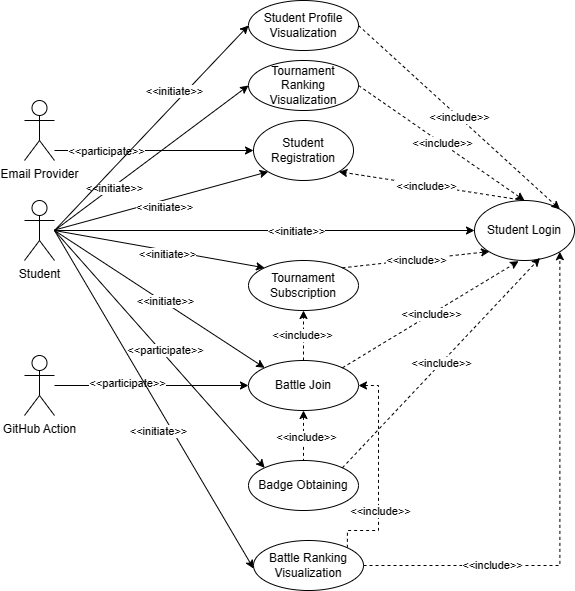
\includegraphics[width=1\linewidth]{Images/UC_Student.png}
    \caption{Student UC Diagram}
    \label{fig:uc_student}
\end{figure}

\newpage

\textbf{Educator Use Case Diagram}
\begin{figure}[H]
    \centering
    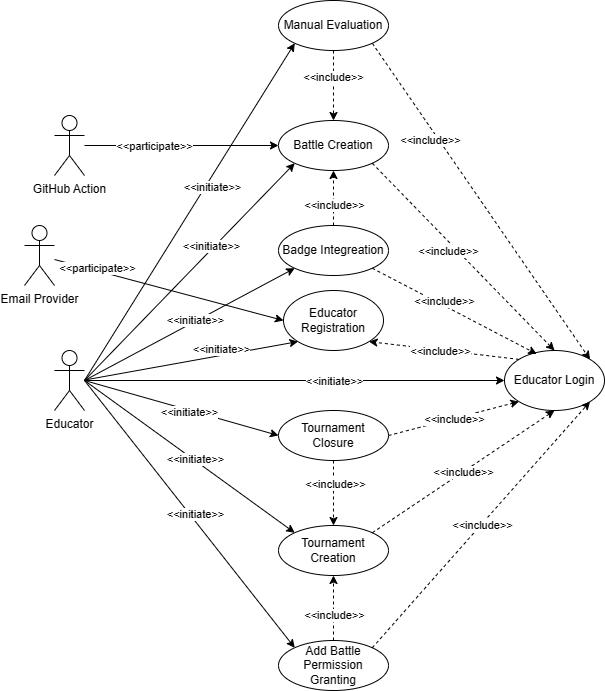
\includegraphics[width=1\linewidth]{Images/UC_Educator.png}
    \caption{Educator UC Diagram}
    \label{fig:uc_educator}
\end{figure}

\newpage

\subsubsection{Sequence diagrams}

\textbf{[UC01] - Student Registration}
\begin{figure}[H]
    \centering
    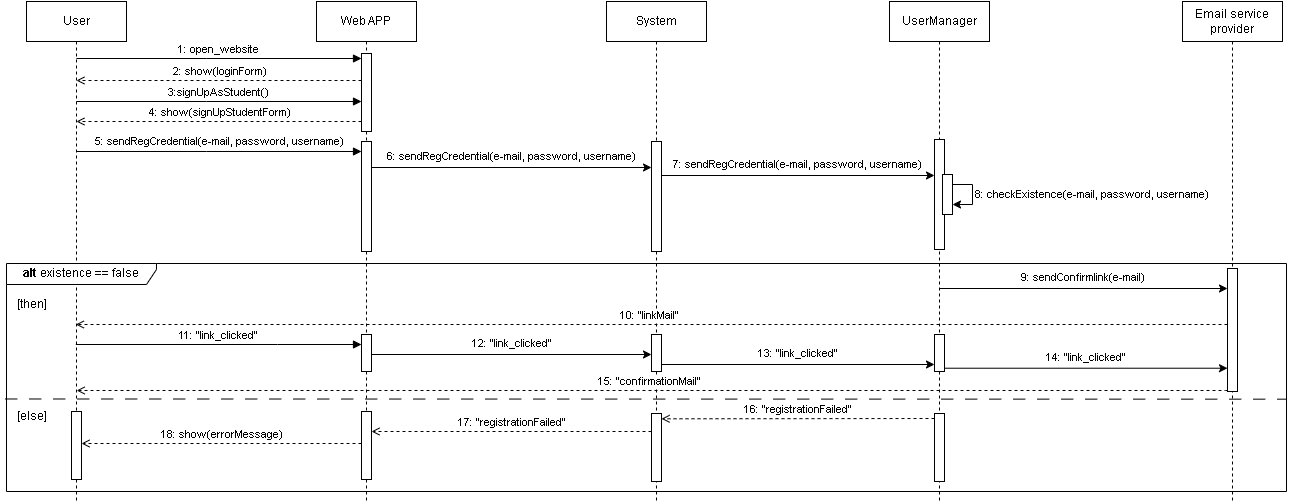
\includegraphics[width=1\linewidth]{Images/SD_StudentRegistration.png}
    \caption{UC01 sequence diagram}
    \label{fig:uc01}
\end{figure}

\textbf{[UC02] - Educator Registration}
\begin{figure}[H]
    \centering
    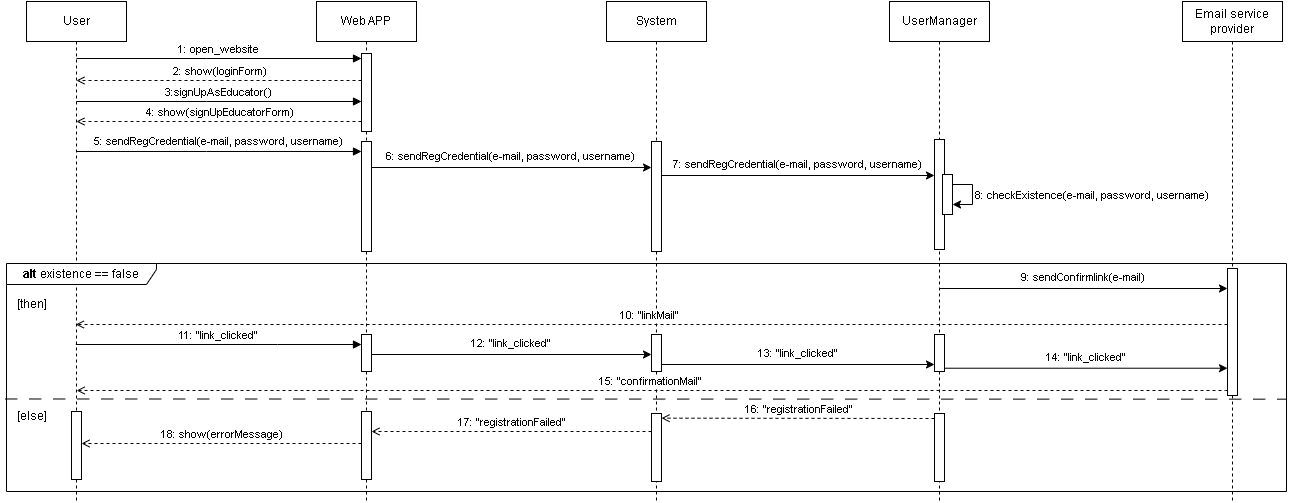
\includegraphics[width=1\linewidth]{Images/SD_EducatorRegistration.png}
    \caption{UC02 sequence diagram}
    \label{fig:uc02}
\end{figure}

\newpage

\textbf{[UC03] - Student login}
\begin{figure}[H]
    \centering
    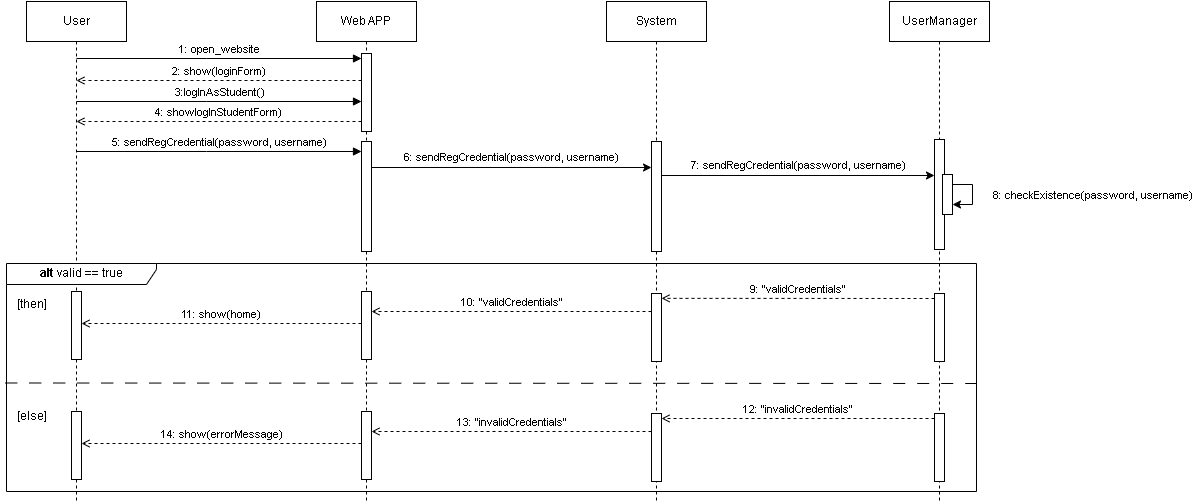
\includegraphics[width=1\linewidth]{Images/SD_StudentLogin.png}
    \caption{UC03 sequence diagram}
    \label{fig:uc03}
\end{figure}

\textbf{[UC04] - Educator login}
\begin{figure}[H]
    \centering
    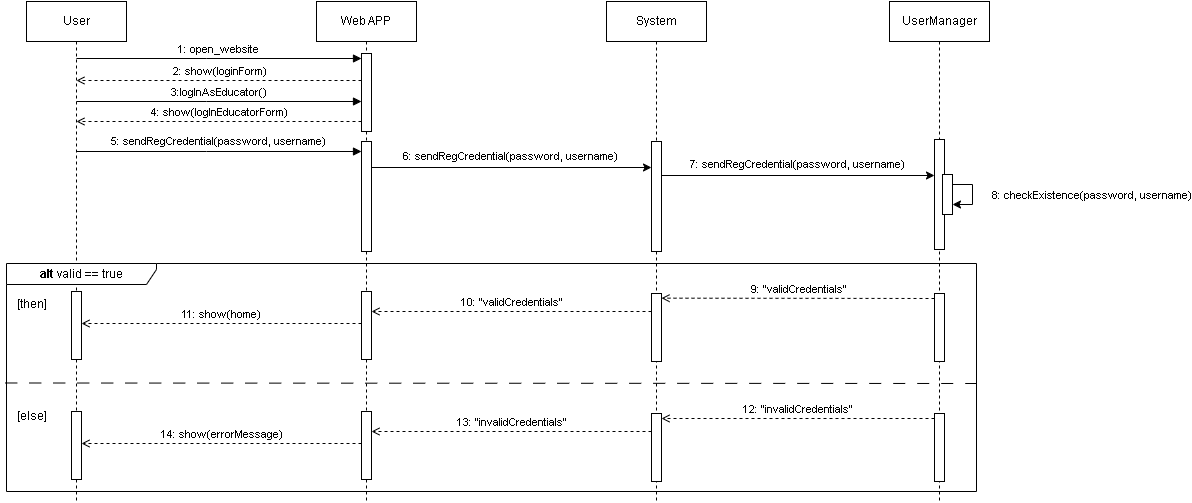
\includegraphics[width=1\linewidth]{Images/SD_EducatorLogin.png}
    \caption{UC04 sequence diagram}
    \label{fig:uc04}
\end{figure}

\newpage

\textbf{[UC05] - Tournament Creation}
\begin{figure}[H]
    \centering
    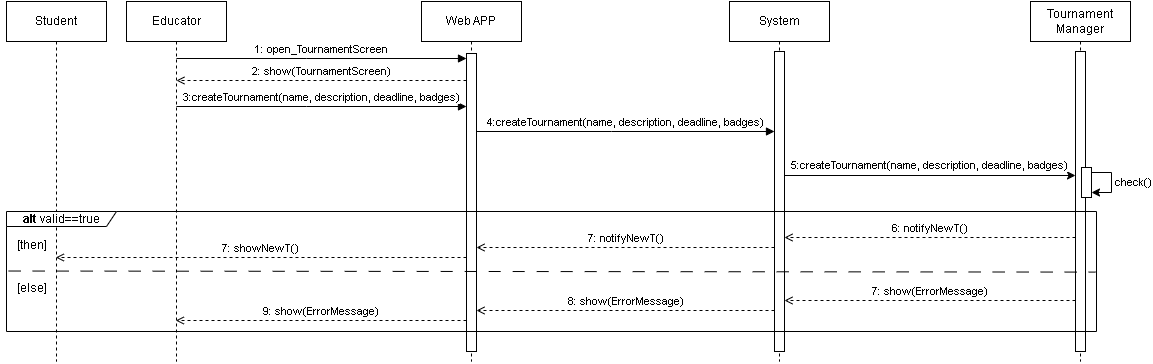
\includegraphics[width=1\linewidth]{Images/SD_TournamentCreation.png}
    \caption{UC05 sequence diagram}
    \label{fig:uc05}
\end{figure}

\textbf{[UC06] - Add Battle Permission Granting}
\begin{figure}[H]
    \centering
    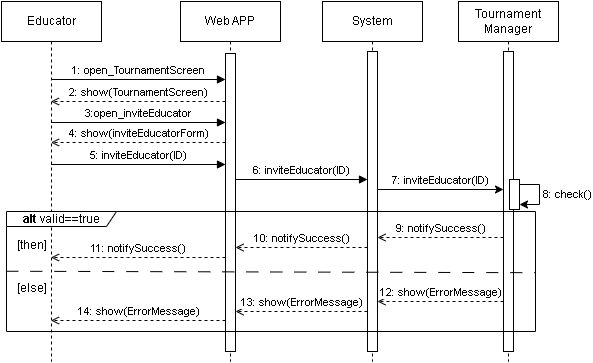
\includegraphics[width=1\linewidth]{Images/SD_AddBattlePermission.png}
    \caption{UC06 sequence diagram}
    \label{fig:uc06}
\end{figure}

\newpage

\textbf{[UC07] - Battle Creation}
\begin{figure}[H]
    \centering
    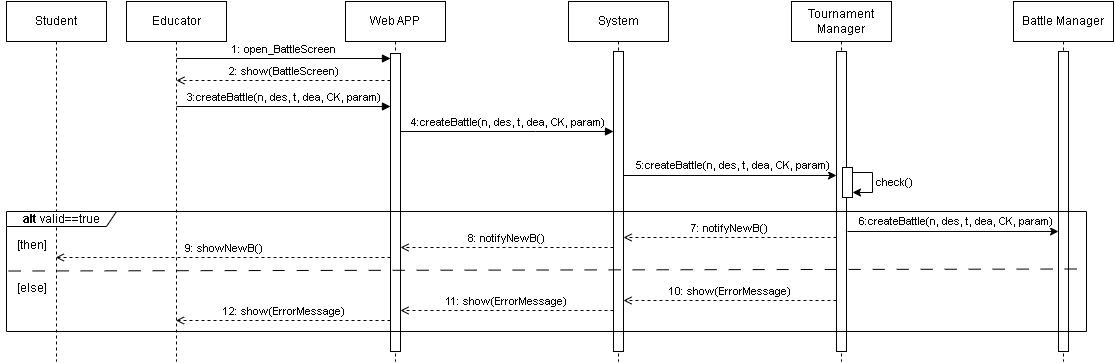
\includegraphics[width=1\linewidth]{Images/SD_BattleCreation.png}
    \caption{UC07 sequence diagram}
    \label{fig:uc07}
\end{figure}

\textbf{[UC08] - Tournament subscription}
\begin{figure}[H]
    \centering
    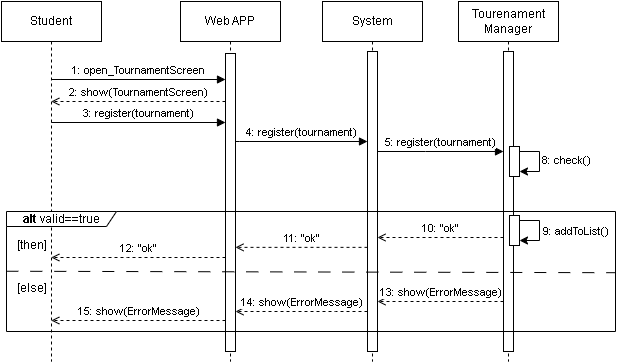
\includegraphics[width=1\linewidth]{Images/SD_TournamentSubscription.png}
    \caption{UC08 sequence diagram}
    \label{fig:uc08}
\end{figure}

\newpage

\textbf{[UC09] - Battle Join}
\begin{figure}[H]
    \centering
    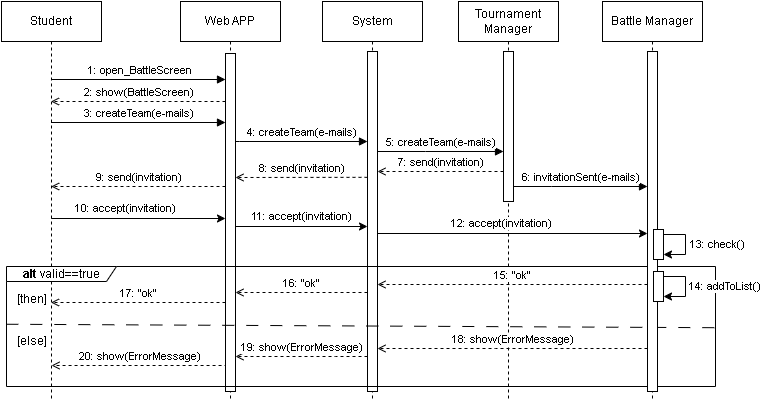
\includegraphics[width=1\linewidth]{Images/SD_BattleJoin.png}
    \caption{UC09 sequence diagram}
    \label{fig:uc09}
\end{figure}

\textbf{[UC10] - Invitation accepting}
\begin{figure}[H]
    \centering
    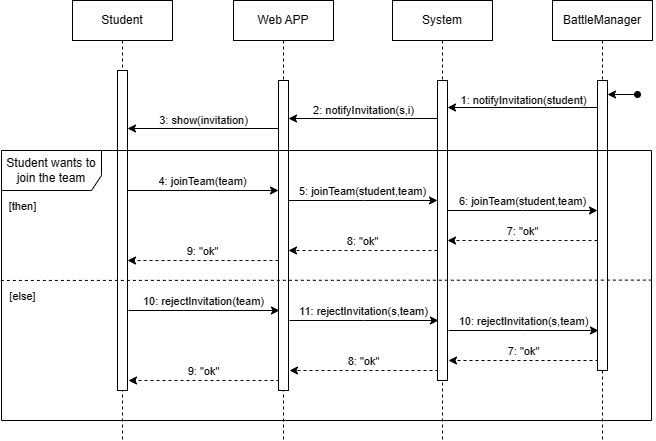
\includegraphics[width=1\linewidth]{Images/SD_Invitation.png}
    \caption{UC10 sequence diagram}
    \label{fig:uc10}
\end{figure}

\newpage

\textbf{[UC11] - Code Manual Evaluation}
\begin{figure}[H]
    \centering
    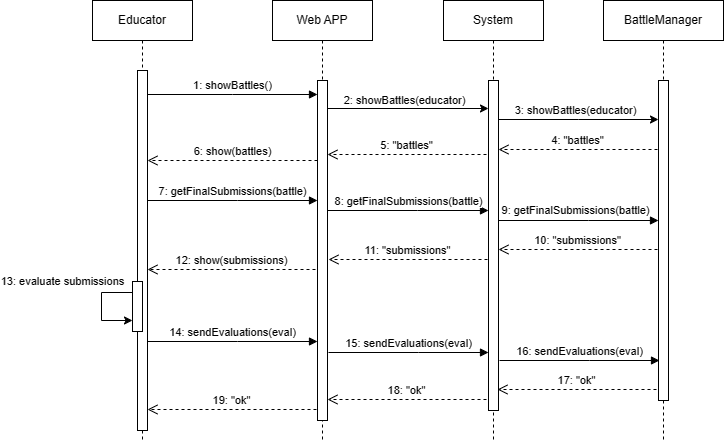
\includegraphics[width=1\linewidth]{Images/SD_ManualEval.png}
    \caption{UC11 sequence diagram}
    \label{fig:uc11}
\end{figure}

\textbf{[UC12] - Tournament Closure}
\begin{figure}[H]
    \centering
    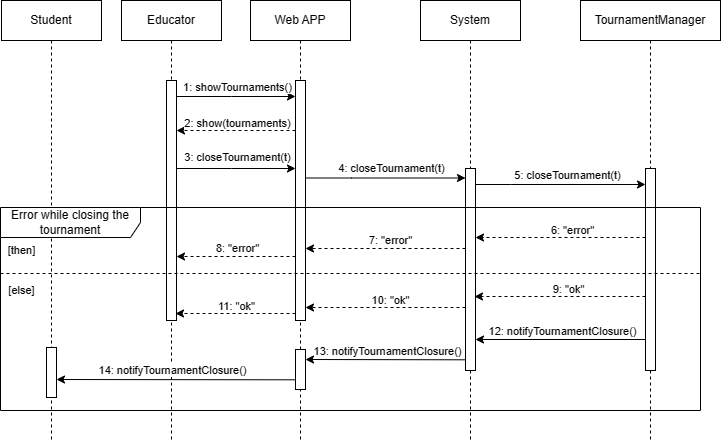
\includegraphics[width=1\linewidth]{Images/SD_TournamentClosure.png}
    \caption{UC12 sequence diagram}
    \label{fig:uc12}
\end{figure}

\newpage

\textbf{[UC13] - Badges Integration}
\begin{figure}[H]
    \centering
    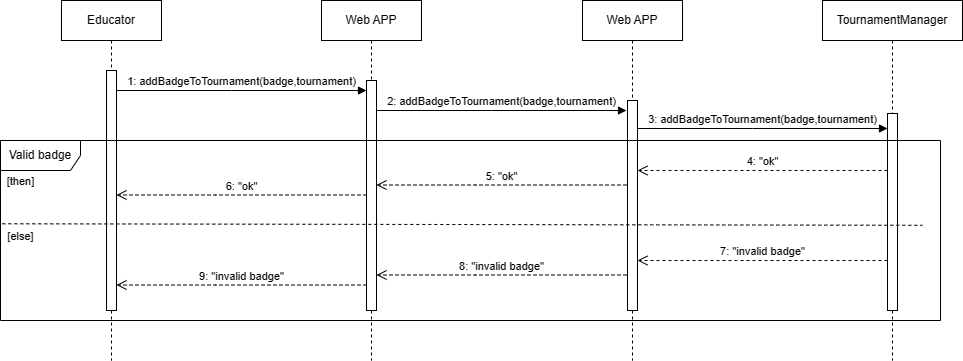
\includegraphics[width=1\linewidth]{Images/SD_BadgeDefinition.png}
    \caption{UC13 sequence diagram}
    \label{fig:uc13}
\end{figure}

\textbf{[UC14] - Badge Obtaining}
\begin{figure}[H]
    \centering
    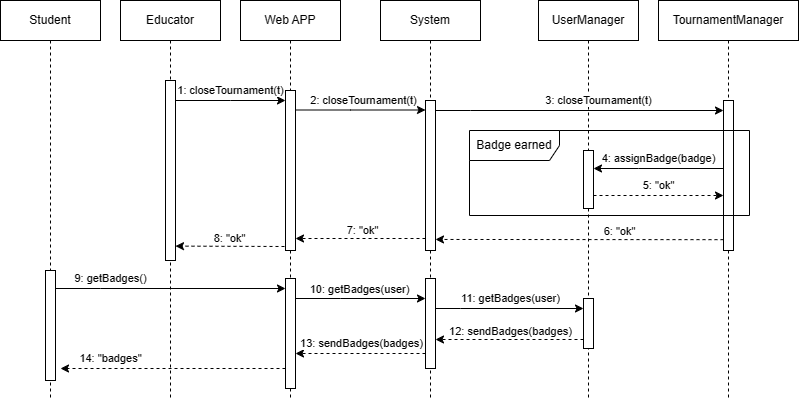
\includegraphics[width=1\linewidth]{Images/SD_BadgeAssignment.png}
    \caption{UC14 sequence diagram}
    \label{fig:uc14}
\end{figure}

\newpage

\textbf{[UC15] - Battle Ranking Visualization}
\begin{figure}[H]
    \centering
    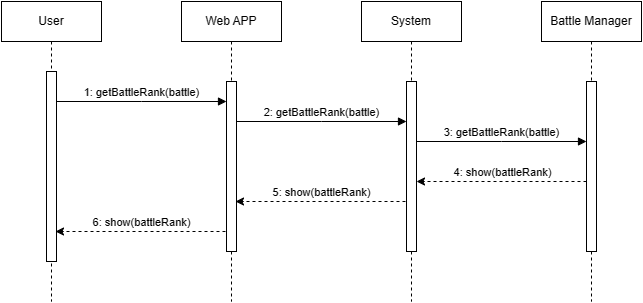
\includegraphics[width=1\linewidth]{Images/SD_BattleRank.png}
    \caption{UC15 sequence diagram}
    \label{fig:uc15}
\end{figure}

\textbf{[UC16] - Tournament Ranking Visualization}
\begin{figure}[H]
    \centering
    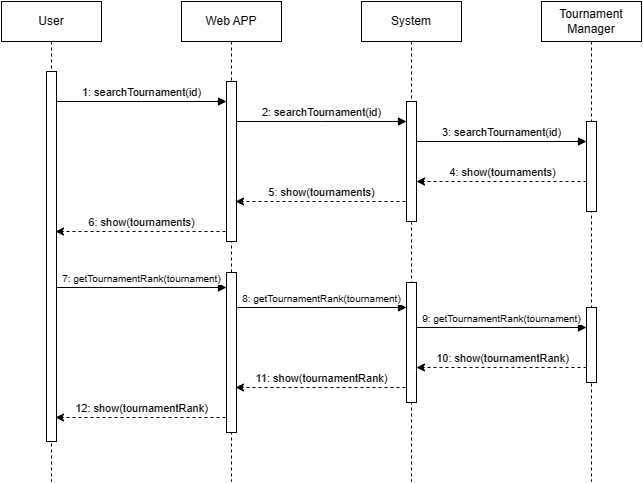
\includegraphics[width=1\linewidth]{Images/SD_TournamentRank.png}
    \caption{UC16 sequence diagram}
    \label{fig:uc16}
\end{figure}

\newpage

\textbf{[UC17] - Student Profile Visualization}
\begin{figure}[H]
    \centering
    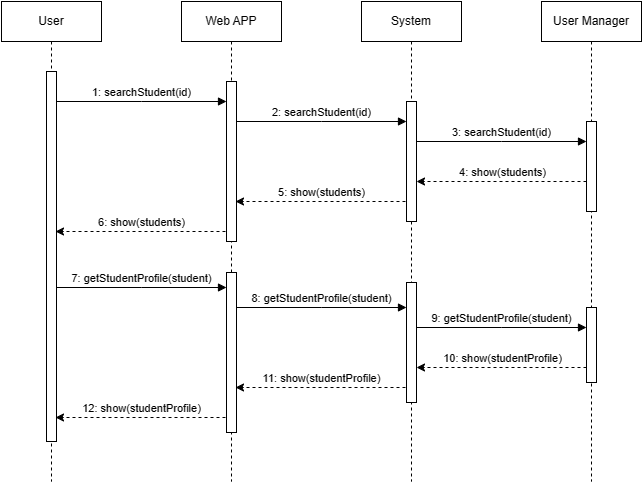
\includegraphics[width=1\linewidth]{Images/SD_StudentProfile.png}
    \caption{UC17 sequence diagram}
    \label{fig:uc17}
\end{figure}

\newpage

\subsubsection{Requirements mapping}

\begin{table}[h!]
    \centering
    \begin{tabular}{|p{8cm}|p{8cm}|}
    \hline
        \multicolumn{2}{|p{16cm}|}{\textbf{[G1] Educator can create tournaments and battles setting all the necessary parameters and badges}} \\
    \hline
        R1: The system must allow users to register on the platform \newline 
        R2: The system must allow users to authenticate themselves and log in securely \newline
        R3: The system must allow educators to create new tournaments \newline
        R4: Tournament creation must include specifying a description of the tournament \newline
        R5: The system must allow authorized educators to create code kata battles within a tournament \newline
        R6: Creation of CKB must include kata description, software project, build scripts, and scoring configurations \newline
        R8: The system automatically creates GitHub repositories for battles \newline
        R14: The system must allow educators to create badges associated with specific tournaments \newline
        R16: The system automatically notifies students and educators about new tournaments, battles, and tournament closures \newline
        R17: Notifications must include deadlines and updates     
        & 
        D1: Users (educators and students) have basic proficiency in using web-based platforms and are familiar with version control systems, such as Git \newline
        D2: Educators have the necessary knowledge to create meaningful code kata battles, including defining test cases and scoring criteria \newline
        D3: Educators and students can connect to the Internet with their devices \newline
        D4: Notification must arrive to connected users in one minute \newline
        D6: Users dispone of an e-mail address \\
    \hline
    \end{tabular}
    \caption{Requirement mapping on goal 1}
    \label{tab:g1}
\end{table}
\begin{table}[h!]
    \centering
    \begin{tabular}{|p{8cm}|p{8cm}|}
    \hline
        \multicolumn{2}{|p{16cm}|}{\textbf{[G2] Student can complete battles on their own or in groups by providing their code}} \\
    \hline
        R1: The system must allow users to register on the platform \newline
        R2: The system must allow users to authenticate themselves and log in securely \newline
        R5: The system must allow educators to create code kata battles within a tournament \newline
        R7: The system must allow students to register for individual battles or form teams based on specified team size limits \newline
        R9: Students must be able to fork the repository and set up automated workflows using GitHub Actions \newline
        R12: The system must allow authorized educators to add battles to tournaments \newline 
        R13: The battle closure triggers updates to personal tournament scores for each student 
        &
        D1: Users (educators and students) have basic proficiency in using web-based platforms and are familiar with version control systems, such as Git \newline 
        D3: Educators and students can connect to the Internet with their devices \newline
        D5: Students are required to have a GitHub account for participation, with the same email address of the CKB account \newline
        D6: Users dispone of an e-mail address \newline
        D7: Users need a reliable internet connection to interact with the CKB platform\newline
        \\
    \hline
    \end{tabular}
    \caption{Requirement mapping on goal 2}
    \label{tab:g2}
\end{table}
\begin{table}[H]
    \centering
    \begin{tabular}{|p{8cm}|p{8cm}|}
    \hline
        \multicolumn{2}{|p{16cm}|}{\textbf{[G3] Educator that creates a tournament can allow other educators to add battles to the tournamen}} \\
    \hline
        R5: The system must allow authorized educators to create code kata battles within a tournament \newline
        R6: Creation of CKB must include kata description, software project, build scripts, and scoring configurations \newline
        R18: The system must allow the educator owning the tournament to authorize other educators to create CKB  
         &
         D3: Educators and students can connect to the Internet with their devices \newline
         D4: Notification must arrive to connected users in one minute \newline
         D6: Users dispone of an e-mail address \\
    \hline
    \end{tabular}
    \caption{Requirement mapping on goal 3}
    \label{tab:g3}
\end{table}
\begin{table}[h!]
    \centering
    \begin{tabular}{|p{8cm}|p{8cm}|}
    \hline
        \multicolumn{2}{|p{16cm}|}{\textbf{[G4] Students and educators can see the list of ongoing and terminated tournaments and the corresponding rank}} \\
    \hline
        R1: The system must allow users to register on the platform \newline
        R2: The system must allow users to authenticate themselves and log in securely \newline
        R10: During the battle, the platform updates scores with every push made by students in real-time \newline
        R11: The system must allow educators to manually evaluate submissions \newline
        R13: The battle closure triggers updates to personal tournament scores for each student
        &
        D3: Educators and students can connect to the Internet with their devices \newline
        D6: Users dispone of an e-mail address \newline
        D7: Users need a reliable internet connection to interact with the CKB platform \newline
        \\
    \hline
    \end{tabular}
    \caption{Requirement mapping on goal 4}
    \label{tab:g4}
\end{table}
\begin{table}[H]
    \centering
    \begin{tabular}{|p{8cm}|p{8cm}|}
    \hline
        \multicolumn{2}{|p{16cm}|}{\textbf{[G5] Students and educators can see the current rank of every battle they are involved in}} \\
    \hline
        R1: The system must allow users to register on the platform \newline
        R2: The system must allow users to authenticate themselves and log in securely \newline
        R10: During the battle, the platform updates scores with every push made by students in real-time \newline
        R13: The battle closure triggers updates to personal tournament scores for each student 
        &
        D3: Educators and students can connect to the Internet with their devices \newline
        D6: Users dispone of an e-mail address \newline
        D7: Users need a reliable internet connection to interact with the CKB platform\\
    \hline
    \end{tabular}
    \caption{Requirement mapping on goal 5}
    \label{tab:g5}
\end{table}
\begin{table}[H]
    \centering
    \begin{tabular}{|p{8cm}|p{8cm}|}
    \hline
        \multicolumn{2}{|p{16cm}|}{\textbf{[G6] Educator can go through the sources produced by a team and manually assign a score}} \\
    \hline
        R1: The system must allow users to register on the platform  \newline
        R2: The system must allow users to authenticate themselves and log in securely \newline
        R11: The system must allow educators to manually evaluate submissions \newline
        R13: The battle closure triggers updates to personal tournament scores for each student \newline
        &
        D1: The users (educators and students) have basic proficiency in using web-based platforms and are familiar with version control systems, such as Git \newline
        D3: Educators and students can connect to the Internet with their devices \newline
        D5: Students are required to have a GitHub account for participation, with the same email address of the CKB account \newline
        D7: Users need a reliable internet connection to interact with the CKB platform\\
    \hline
    \end{tabular}
    \caption{Requirement mapping on goal 6}
    \label{tab:g6}
\end{table}
\begin{table}[H]
    \centering
    \begin{tabular}{|p{8cm}|p{8cm}|}
    \hline
        \multicolumn{2}{|p{16cm}|}{\textbf{[G7] Educators and students can visualize all badges and every student’s collected badges}} \\
    \hline
        R14: The system must allow educators to create badges associated with specific tournaments \newline
        R15: Badges are automatically assigned based on predefined rules and student performance \newline
        &
        D3: Educators and students can connect to the Internet with their devices \newline 
        D6: Users dispone of an e-mail address \\
    \hline
    \end{tabular}
    \caption{Requirement mapping on goal 7}
    \label{tab:g7}
\end{table}

\newpage

\subsection{Performance requirements}
\begin{enumerate}
  \item \textbf{Response time:} \\
  To ensure timely responsiveness for user interactions the platform should respond to user actions (e.g., loading pages, submitting forms) within a maximum of two seconds under normal load conditions.
  \item \textbf{Scalability:} \\
  To ensure the platform can handle an increasing number of users and data the platform should support concurrent access by at least 1000 users without significant degradation in performance, for up to 1000 battles simultaneously.
  \item \textbf{GitHub integration:} \\
  GitHub repository creation, including code kata and automation setup, should take no longer than two minutes, also automated workflow triggers from GHA should result in platform updates within 1 minute of code submission, otherwise, some students’ submission may be lost.
  \item \textbf{Automated assessment and consolidation stage:} \\
  To ensure fast evaluation of code submissions, automated assessments (including code analysis and test execution) should complete within two minutes for a battle. Also, the platform should handle simultaneous automated assessments from multiple battles without queuing delays.
  \item \textbf{Notification system:} \\
  Notifications about battle and tournament updates need to be sent to every interested user in at most one minute.
  \item \textbf{Badges and gamification:} \\
  To provide a continuous experience for badge assignment and visualization, they need to be assigned right after the end of each tournament and to the correct students. Also, their visualization on users’ profile should load instantaneously.
  \item \textbf{Security:} \\
  To ensure secure data handling and prevent unauthorized access user authentication and authorization processes should happen rapidly and the platform should do regular security inspections to identify and address potential vulnerabilities.
  \item \textbf{Data storage and retrieval:} \\
  To optimize data storage and retrieval processes, database queries for common operations should be fully optimized. Frequent backups are done to prevent data losses.
  \item \textbf{Reliability:} \\
  To ensure consistent and reliable performance, the platform should achieve 99.9\% uptime.
\end{enumerate}
These are criteria that CKB aims to achieve. Rigorous testing and continuous monitoring will be essential to meet and maintain these standards throughout the system’s lifecycle.

\subsection{Design constraints}
These are the constraints related to the design of the system. They are divided in three
categories: standards compliance, hardware limitations and other constraints.

\subsubsection{Standard compliance}
\begin{enumerate}
  \item \textbf{Web standards:} \\ 
  User interface and interactions must adhere to modern web standards, ensuring compatibility with major web browsers such as Chrome, Firefox, Safari, and Edge.
  \item \textbf{Coding standards:} \\
  Code written for the platform must stick to standard coding conventions, such as proper documentation and modular design.
  \item \textbf{Security standards:} \\
  The platform must comply with standard security protocols to safeguard user data, prevent unauthorized access and protect against common web vulnerabilities, e.g. Cross-Site Scripting, File Inclusion Vulnerabilities or injection attacks.
  \item \textbf{Data privacy regulations:} \\
  The platform must comply with data privacy regulations  such as General Data Protection Regulation (GDPR) and California Consumer Privacy Act (CCPA), and ensure the secure handling of user data, in addition, explicit consent must be obtained from users regarding data collection and usage.
  \item \textbf{Environmental sustainability for servers:} \\
  Servers hosting the platform need to adhere to the most recent environmental sustainability standards. This includes considerations for energy efficiency, eco-friendly practices, and responsible disposal of electronic waste.
\end{enumerate}

\subsubsection{Hardware limitations}
\begin{enumerate}
  \item \textbf{Server requirements:} \\
  The platform's server infrastructure must meet the specified minimum requirements for processing power, memory and storage to ensure optimal performance and responsiveness.
  \item \textbf{Internet connection:} \\
  Users accessing the platform must have a reliable and high-speed internet connection to ensure efficient participation in battles, timely submission of solutions and access to real-time updates.
\end{enumerate}

\subsubsection{Any other constraints}
\begin{enumerate}
  \item \textbf{Educator access:} \\
  Educators must have appropriate permissions to create and manage tournaments, battles and associated configurations. Access control mechanisms must be in place via discretionary access control to prevent unauthorized access.
  \item \textbf{GitHub integration:} \\
  Users must have a GitHub account to fully utilize the platform's features, especially the integration with GitHub repositories and automated workflows.
  \item \textbf{GitHub API rate limits:} \\
  The platform must adhere to GitHub's API rate limits to avoid disruptions in GitHub integration. Excessive API requests may result in rate-limiting, affecting the automated workflow triggered by code submissions.
  \item \textbf{Scalability considerations:} \\
  Scaling beyond a certain threshold may lead to additional costs or require adjustments to the hosting environment.
\end{enumerate}

\subsection{Software System Attributes}
\subsubsection{Reliability}
The platform must consistently and accurately perform its functions without failures or errors. To do so is necessary to implement error handling mechanisms and use a redundant system to ensure continuous operation. \\
Also to not lose data in case of a failure it’s necessary to frequently back up all the data in the database, keeping them in a different building and offline to their security. \\
It’s also important to test the whole system, including unit testing and integration testing, to identify and correct bugs and malfunctioning.

\subsubsection{Availability}
The platform must be accessible to users when needed. A way to assure that is to implement a physical load balancing system that distributes incoming traffic through different server’s replicas to prevent overload. Server’s and data center’s replicas also permit to minimize downtime in case of hardware failures. The usage of monitoring tools can also be very helpful to detect and respond to issues, ensuring high system uptime. \\
Since this system does not provide emergency services or services related to critical situations, it must provide availability of 99.9\%. To have the best results, it is essential that the Mean Time To Failures (MTTF) is as long as possible and that the Mean Time to Repair (MTTR) is as short as possible.

\subsubsection{Security}
To safeguard the platform against unauthorized access, data breaches and malicious activities, it’s necessary to employ an encryption mechanism to protect data during transmission (avoiding attacks like sniffing and spoofing) and storage in the database, also to guarantee users’ privacy. Developers need to implement secure coding practices to mitigate vulnerabilities such as injection attacks (e.g. SQL injection), cross-site scripting (XSS) and cross-site request forgery (CSRF), at application level a Web Application Firewall (WAF) is employed to protect against this common attacks and also to log and alert on suspicious activities, providing insights for threat response. \\
Also, since the script uploaded can be potentially dangerous to execute on servers, it’s necessary to implement a robust sandboxing mechanism to isolate and execute user-uploaded code securely, can also be very helpful the usage of static code analysis tools and threat intelligence feeds and pattern matching to check user-submitted code for potential security vulnerabilities or malicious code patterns before execution. Another important thing is applying restrictions on resource usage (CPU, memory) to prevent malicious activities from the users. \\
At physical level are necessary infrastructures such as: firewalls that filter and monitor incoming network traffic, Intrusion Detection System (IDS) to detect and respond to security threats or unusual activities. \\
Finally, frequently conduct regular checks and reviews for security and vulnerability and penetration testing to identify and address potential weaknesses is fundamental.

\subsubsection{Maintainability}
The platform should be easily modified, updated and widened over its lifecycle. Some approaches can be adopting modular code structures to facilitate code maintenance and utilizing version control systems for tracking changes and managing collaborative development, also it’s important the incorporation of an automated testing routine that covers at least the 75\% of the code and the continuous update of the software.

\subsubsection{Portability}
The platform needs to run on different environments and platforms. The principal solution is to implement platform-independent code by adhering to standard programming languages and frameworks, also it’s necessary to address dependencies and ensure compatibility with different operating systems and web browsers, this can be done using containerization technologies (e.g. Docker) for packaging and deploying applications consistently across various environments.